\documentclass[12pt]{article}

%** Package ****************************************************************************************

%**** Page settings ******************************

\usepackage[%
paper=a0paper,%
%landscape,
%includeheadfoot,%
margin=10mm,%
headsep=0cm, footskip=0cm,%
dvips,%
]{geometry}

%**** Encoding ***********************************

\usepackage[utf8]{inputenc}

%*************************************************

\usepackage{tikz}
\usetikzlibrary{calc}
\usepgflibrary{arrows}

\usepackage{calc}

%***************************************************************************************************

\begin{document}
\pagestyle{empty}
\fontsize{64}{72}\selectfont % \fontsize{size}{baselineskip}
\begin{center}
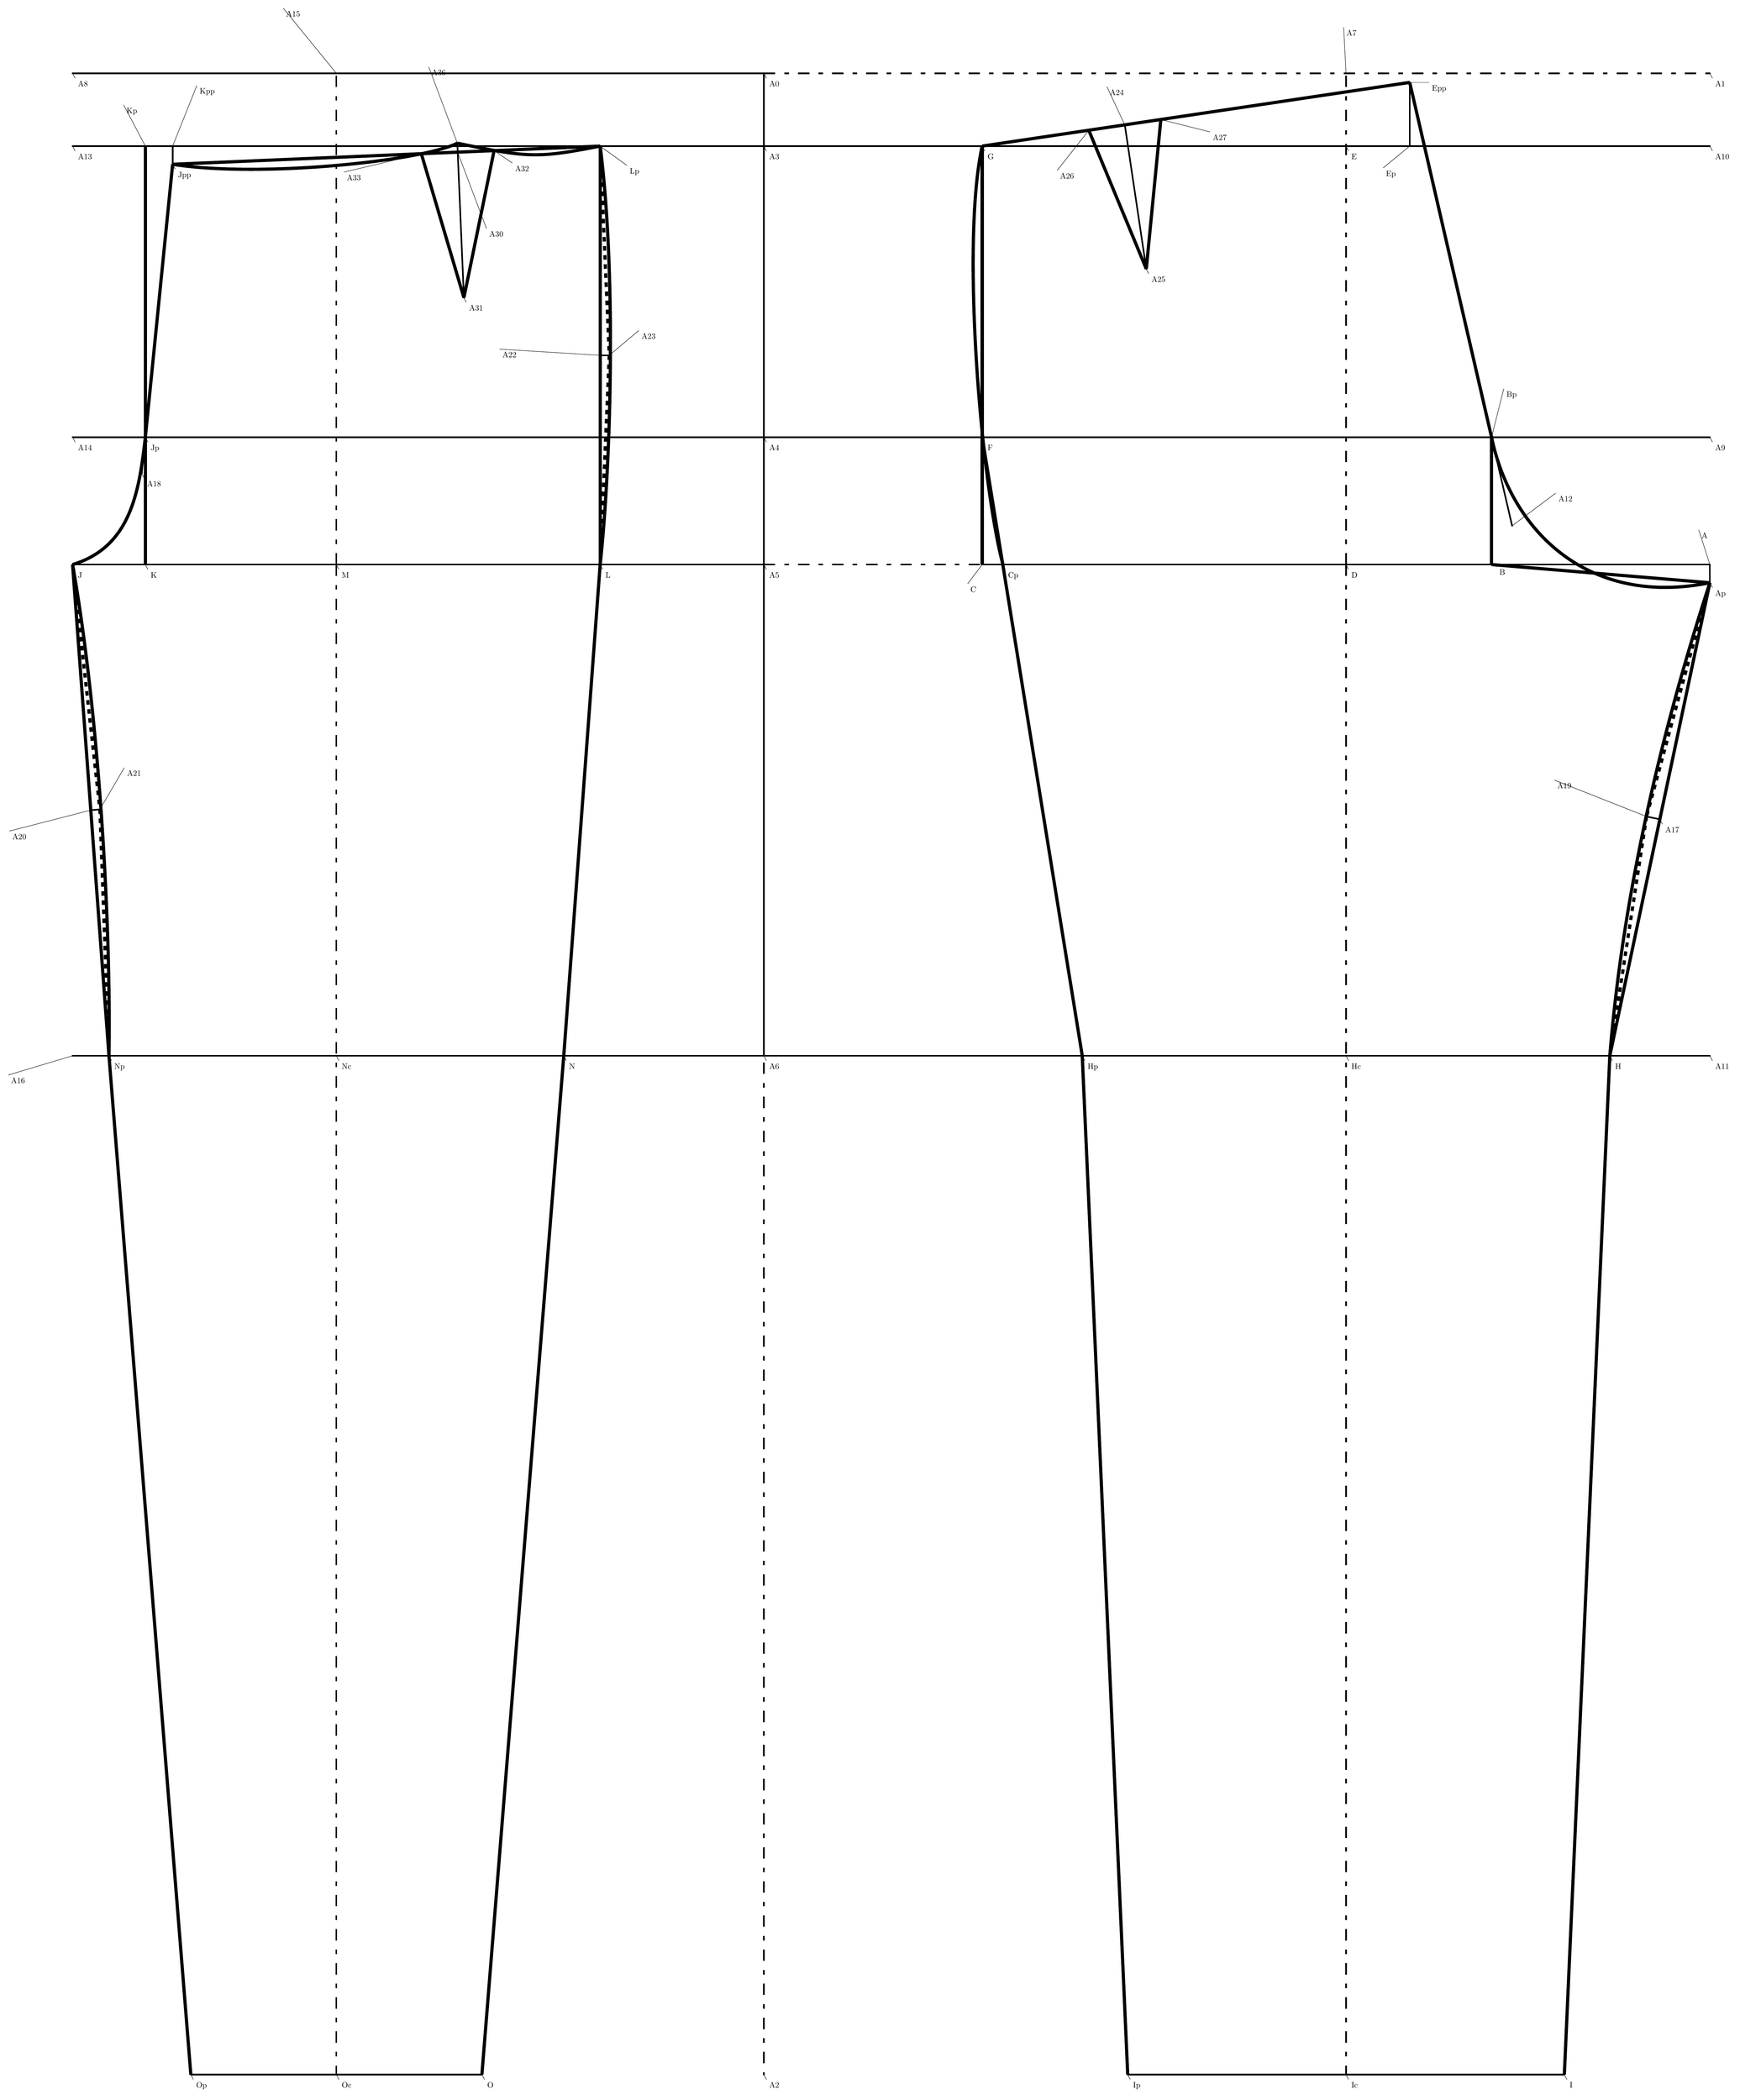
\begin{tikzpicture}[x=8mm,y=8mm]
\coordinate (A0) at (0.79,1.06);
\fill [black] (A0) circle (1pt);
\draw[line width=.5pt] (0.79,1.06) -- (0.93,0.79);
\draw[] (0.93,0.79) node[anchor=north west] {A0};
\coordinate (A1) at (52.79,1.06);
\fill [black] (A1) circle (1pt);
\draw[line width=.5pt] (52.79,1.06) -- (52.93,0.79);
\draw[] (52.93,0.79) node[anchor=north west] {A1};
\draw[line width=2pt, dash pattern=on 5mm off 4mm on 2mm off 4mm, black] (A0) -- (A1);
\coordinate (A2) at (0.79,-108.94);
\fill [black] (A2) circle (1pt);
\draw[line width=.5pt] (0.79,-108.94) -- (0.93,-109.21);
\draw[] (0.93,-109.21) node[anchor=north west] {A2};
\draw[line width=2pt, dash pattern=on 5mm off 4mm on 2mm off 4mm, black] (A0) -- (A2);
\coordinate (A3) at (0.79,-2.94);
\fill [black] (A3) circle (1pt);
\draw[line width=.5pt] (0.79,-2.94) -- (0.93,-3.21);
\draw[] (0.93,-3.21) node[anchor=north west] {A3};
\draw[line width=2pt, black] (A0) -- (A3);
\coordinate (A4) at (0.79,-18.94);
\fill [black] (A4) circle (1pt);
\draw[line width=.5pt] (0.79,-18.94) -- (0.93,-19.21);
\draw[] (0.93,-19.21) node[anchor=north west] {A4};
\draw[line width=2pt, black] (A0) -- (A4);
\coordinate (A5) at (0.79,-25.94);
\fill [black] (A5) circle (1pt);
\draw[line width=.5pt] (0.79,-25.94) -- (0.93,-26.21);
\draw[] (0.93,-26.21) node[anchor=north west] {A5};
\draw[line width=2pt, black] (A0) -- (A5);
\coordinate (A6) at (0.79,-52.94);
\fill [black] (A6) circle (1pt);
\draw[line width=.5pt] (0.79,-52.94) -- (0.93,-53.21);
\draw[] (0.93,-53.21) node[anchor=north west] {A6};
\draw[line width=2pt, black] (A0) -- (A6);
\coordinate (A) at (52.79,-25.94);
\fill [black] (A) circle (1pt);
\draw[line width=.5pt] (52.79,-25.94) -- (52.18,-24.04);
\draw[] (52.18,-24.04) node[anchor=north west] {A};
\draw[line width=2pt, dash pattern=on 5mm off 4mm on 2mm off 4mm, black] (A5) -- (A);
\coordinate (B) at (40.79,-25.94);
\fill [black] (B) circle (1pt);
\draw[line width=.5pt] (40.79,-25.94) -- (41.07,-26.06);
\draw[] (41.07,-26.06) node[anchor=north west] {B};
\draw[line width=2pt, solid, black] (A) -- (B);
\coordinate (C) at (12.79,-25.94);
\fill [black] (C) circle (1pt);
\draw[line width=.5pt] (12.79,-25.94) -- (11.99,-27.00);
\draw[] (11.99,-27.00) node[anchor=north west] {C};
\draw[line width=2pt, solid, black] (B) -- (C);
\coordinate (D) at (32.79,-25.94);
\fill [black] (D) circle (1pt);
\draw[line width=.5pt] (32.79,-25.94) -- (32.93,-26.21);
\draw[] (32.93,-26.21) node[anchor=north west] {D};
\draw[line width=2pt, solid, black] (C) -- (D);
\coordinate (A7) at (32.79,1.06);
\fill [black] (A7) circle (1pt);
\draw[line width=.5pt] (32.79,1.06) -- (32.66,3.59);
\draw[] (32.66,3.59) node[anchor=north west] {A7};
\draw[line width=2pt, dash pattern=on 5mm off 4mm on 2mm off 4mm, black] (D) -- (A7);
\coordinate (Ic) at (32.79,-108.94);
\fill [black] (Ic) circle (1pt);
\draw[line width=.5pt] (32.79,-108.94) -- (32.93,-109.21);
\draw[] (32.93,-109.21) node[anchor=north west] {Ic};
\draw[line width=2pt, dash pattern=on 5mm off 4mm on 2mm off 4mm, black] (D) -- (Ic);
\coordinate (A9) at (52.79,-18.94);
\fill [black] (A9) circle (1pt);
\draw[line width=.5pt] (52.79,-18.94) -- (52.93,-19.21);
\draw[] (52.93,-19.21) node[anchor=north west] {A9};
\draw[line width=2pt, solid, black] (A4) -- (A9);
\coordinate (A10) at (52.79,-2.94);
\fill [black] (A10) circle (1pt);
\draw[line width=.5pt] (52.79,-2.94) -- (52.93,-3.21);
\draw[] (52.93,-3.21) node[anchor=north west] {A10};
\draw[line width=2pt, solid, black] (A3) -- (A10);
\coordinate (A11) at (52.79,-52.94);
\fill [black] (A11) circle (1pt);
\draw[line width=.5pt] (52.79,-52.94) -- (52.93,-53.21);
\draw[] (52.93,-53.21) node[anchor=north west] {A11};
\draw[line width=2pt, solid, black] (A6) -- (A11);
\coordinate (E) at (32.79,-2.94);
\fill [black] (E) circle (1pt);
\draw[line width=.5pt] (32.79,-2.94) -- (32.93,-3.21);
\draw[] (32.93,-3.21) node[anchor=north west] {E};
\coordinate (Ep) at (36.29,-2.94);
\fill [black] (Ep) circle (1pt);
\draw[line width=.5pt] (36.29,-2.94) -- (34.83,-4.14);
\draw[] (34.83,-4.14) node[anchor=north west] {Ep};
\draw[line width=2pt, black] (E) -- (Ep);
\coordinate (Epp) at (36.29,0.56);
\fill [black] (Epp) circle (1pt);
\draw[line width=.5pt] (36.29,0.56) -- (37.36,0.56);
\draw[] (37.36,0.56) node[anchor=north west] {Epp};
\draw[line width=2pt, solid, black] (Ep) -- (Epp);
\coordinate (Ap) at (52.79,-26.94);
\fill [black] (Ap) circle (1pt);
\draw[line width=.5pt] (52.79,-26.94) -- (52.93,-27.21);
\draw[] (52.93,-27.21) node[anchor=north west] {Ap};
\draw[line width=2pt, solid, black] (A) -- (Ap);
\coordinate (Bp) at (40.79,-18.94);
\fill [black] (Bp) circle (1pt);
\draw[line width=.5pt] (40.79,-18.94) -- (41.46,-16.28);
\draw[] (41.46,-16.28) node[anchor=north west] {Bp};
\draw[line width=4pt, solid, black] (Ap) -- (B);
\draw[line width=4pt, solid, black] (Epp) -- (Bp);
\draw[line width=4pt, solid, black] (Bp) -- (B);
\draw[line width=4pt, solid, black] (Bp) .. controls (41.82,-23.93) and (45.95,-28.31) .. (Ap);
\coordinate (A12) at (41.92,-23.81);
\fill [black] (A12) circle (1pt);
\draw[line width=.5pt] (41.92,-23.81) -- (44.31,-22.02);
\draw[] (44.31,-22.02) node[anchor=north west] {A12};
\draw[line width=2pt, black] (Bp) -- (A12);
\coordinate (F) at (12.79,-18.94);
\fill [black] (F) circle (1pt);
\draw[line width=.5pt] (12.79,-18.94) -- (12.93,-19.21);
\draw[] (12.93,-19.21) node[anchor=north west] {F};
\draw[line width=2pt, black] (Bp) -- (F);
\coordinate (G) at (12.79,-2.94);
\fill [black] (G) circle (1pt);
\draw[line width=.5pt] (12.79,-2.94) -- (12.93,-3.21);
\draw[] (12.93,-3.21) node[anchor=north west] {G};
\draw[line width=4pt, solid, black] (G) -- (Epp);
\coordinate (Hc) at (32.79,-52.94);
\fill [black] (Hc) circle (1pt);
\draw[line width=.5pt] (32.79,-52.94) -- (32.93,-53.21);
\draw[] (32.93,-53.21) node[anchor=north west] {Hc};
\coordinate (H) at (47.29,-52.94);
\fill [black] (H) circle (1pt);
\draw[line width=.5pt] (47.29,-52.94) -- (47.43,-53.21);
\draw[] (47.43,-53.21) node[anchor=north west] {H};
\draw[line width=2pt, black] (Hc) -- (H);
\coordinate (Hp) at (18.29,-52.94);
\fill [black] (Hp) circle (1pt);
\draw[line width=.5pt] (18.29,-52.94) -- (18.43,-53.21);
\draw[] (18.43,-53.21) node[anchor=north west] {Hp};
\draw[line width=2pt, black] (Hc) -- (Hp);
\coordinate (Ip) at (20.79,-108.94);
\fill [black] (Ip) circle (1pt);
\draw[line width=.5pt] (20.79,-108.94) -- (20.93,-109.21);
\draw[] (20.93,-109.21) node[anchor=north west] {Ip};
\draw[line width=2pt, solid, black] (Ic) -- (Ip);
\coordinate (I) at (44.79,-108.94);
\fill [black] (I) circle (1pt);
\draw[line width=.5pt] (44.79,-108.94) -- (44.93,-109.21);
\draw[] (44.93,-109.21) node[anchor=north west] {I};
\draw[line width=2pt, solid, black] (Ip) -- (I);
\draw[line width=4pt, solid, black] (Ip) -- (Hp);
\draw[line width=4pt, solid, black] (H) -- (I);
\draw[line width=4pt, solid, black] (Hp) -- (F);
\draw[line width=4pt, solid, black] (H) -- (Ap);
\coordinate (Cp) at (13.93,-25.94);
\fill [black] (Cp) circle (1pt);
\draw[line width=.5pt] (13.93,-25.94) -- (14.06,-26.21);
\draw[] (14.06,-26.21) node[anchor=north west] {Cp};
\draw[line width=4pt, solid, black] (F) -- (G);
\draw[line width=4pt, solid, black] (C) -- (F);
\coordinate (A8) at (-37.21,1.06);
\fill [black] (A8) circle (1pt);
\draw[line width=.5pt] (-37.21,1.06) -- (-37.07,0.79);
\draw[] (-37.07,0.79) node[anchor=north west] {A8};
\draw[line width=2pt, solid, black] (A0) -- (A8);
\coordinate (A13) at (-37.21,-2.94);
\fill [black] (A13) circle (1pt);
\draw[line width=.5pt] (-37.21,-2.94) -- (-37.07,-3.21);
\draw[] (-37.07,-3.21) node[anchor=north west] {A13};
\draw[line width=2pt, solid, black] (A3) -- (A13);
\coordinate (A14) at (-37.21,-18.94);
\fill [black] (A14) circle (1pt);
\draw[line width=.5pt] (-37.21,-18.94) -- (-37.07,-19.21);
\draw[] (-37.07,-19.21) node[anchor=north west] {A14};
\draw[line width=2pt, solid, black] (A4) -- (A14);
\coordinate (J) at (-37.21,-25.94);
\fill [black] (J) circle (1pt);
\draw[line width=.5pt] (-37.21,-25.94) -- (-37.07,-26.21);
\draw[] (-37.07,-26.21) node[anchor=north west] {J};
\draw[line width=2pt, solid, black] (A5) -- (J);
\coordinate (A16) at (-37.21,-52.94);
\fill [black] (A16) circle (1pt);
\draw[line width=.5pt] (-37.21,-52.94) -- (-40.75,-54.00);
\draw[] (-40.75,-54.00) node[anchor=north west] {A16};
\draw[line width=2pt, solid, black] (A6) -- (A16);
\coordinate (K) at (-33.21,-25.94);
\fill [black] (K) circle (1pt);
\draw[line width=.5pt] (-33.21,-25.94) -- (-33.07,-26.21);
\draw[] (-33.07,-26.21) node[anchor=north west] {K};
\draw[line width=2pt, black] (J) -- (K);
\coordinate (L) at (-8.21,-25.94);
\fill [black] (L) circle (1pt);
\draw[line width=.5pt] (-8.21,-25.94) -- (-8.07,-26.21);
\draw[] (-8.07,-26.21) node[anchor=north west] {L};
\draw[line width=2pt, black] (K) -- (L);
\coordinate (M) at (-22.71,-25.94);
\fill [black] (M) circle (1pt);
\draw[line width=.5pt] (-22.71,-25.94) -- (-22.57,-26.21);
\draw[] (-22.57,-26.21) node[anchor=north west] {M};
\draw[line width=2pt, black] (L) -- (M);
\coordinate (A15) at (-22.71,1.06);
\fill [black] (A15) circle (1pt);
\draw[line width=.5pt] (-22.71,1.06) -- (-25.63,4.64);
\draw[] (-25.63,4.64) node[anchor=north west] {A15};
\draw[line width=2pt, dash pattern=on 5mm off 4mm on 2mm off 4mm, black] (M) -- (A15);
\coordinate (Oc) at (-22.71,-108.94);
\fill [black] (Oc) circle (1pt);
\draw[line width=.5pt] (-22.71,-108.94) -- (-22.57,-109.21);
\draw[] (-22.57,-109.21) node[anchor=north west] {Oc};
\draw[line width=2pt, dash pattern=on 5mm off 4mm on 2mm off 4mm, black] (M) -- (Oc);
\coordinate (Kp) at (-33.21,-2.94);
\fill [black] (Kp) circle (1pt);
\draw[line width=.5pt] (-33.21,-2.94) -- (-34.40,-0.68);
\draw[] (-34.40,-0.68) node[anchor=north west] {Kp};
\coordinate (Lp) at (-8.21,-2.94);
\fill [black] (Lp) circle (1pt);
\draw[line width=.5pt] (-8.21,-2.94) -- (-6.74,-4.00);
\draw[] (-6.74,-4.00) node[anchor=north west] {Lp};
\draw[line width=4pt, solid, black] (K) -- (Kp);
\draw[line width=4pt, solid, black] (L) -- (Lp);
\coordinate (Jp) at (-33.21,-18.94);
\fill [black] (Jp) circle (1pt);
\draw[line width=.5pt] (-33.21,-18.94) -- (-33.07,-19.21);
\draw[] (-33.07,-19.21) node[anchor=north west] {Jp};
\coordinate (Kpp) at (-31.71,-2.94);
\fill [black] (Kpp) circle (1pt);
\draw[line width=.5pt] (-31.71,-2.94) -- (-30.38,0.39);
\draw[] (-30.38,0.39) node[anchor=north west] {Kpp};
\draw[line width=2pt, black] (Kp) -- (Kpp);
\coordinate (Jpp) at (-31.71,-3.94);
\fill [black] (Jpp) circle (1pt);
\draw[line width=.5pt] (-31.71,-3.94) -- (-31.57,-4.21);
\draw[] (-31.57,-4.21) node[anchor=north west] {Jpp};
\draw[line width=2pt, solid, black] (Kpp) -- (Jpp);
\draw[line width=4pt, solid, black] (Jpp) -- (Lp);
\draw[line width=4pt, solid, black] (Jpp) -- (Jp);
\coordinate (Nc) at (-22.71,-52.94);
\fill [black] (Nc) circle (1pt);
\draw[line width=.5pt] (-22.71,-52.94) -- (-22.57,-53.21);
\draw[] (-22.57,-53.21) node[anchor=north west] {Nc};
\coordinate (N) at (-10.21,-52.94);
\fill [black] (N) circle (1pt);
\draw[line width=.5pt] (-10.21,-52.94) -- (-10.07,-53.21);
\draw[] (-10.07,-53.21) node[anchor=north west] {N};
\draw[line width=2pt, black] (Nc) -- (N);
\coordinate (Np) at (-35.21,-52.94);
\fill [black] (Np) circle (1pt);
\draw[line width=.5pt] (-35.21,-52.94) -- (-35.07,-53.21);
\draw[] (-35.07,-53.21) node[anchor=north west] {Np};
\draw[line width=2pt, black] (Nc) -- (Np);
\coordinate (O) at (-14.71,-108.94);
\fill [black] (O) circle (1pt);
\draw[line width=.5pt] (-14.71,-108.94) -- (-14.57,-109.21);
\draw[] (-14.57,-109.21) node[anchor=north west] {O};
\draw[line width=2pt, black] (Oc) -- (O);
\coordinate (Op) at (-30.71,-108.94);
\fill [black] (Op) circle (1pt);
\draw[line width=.5pt] (-30.71,-108.94) -- (-30.57,-109.21);
\draw[] (-30.57,-109.21) node[anchor=north west] {Op};
\draw[line width=2pt, solid, black] (O) -- (Op);
\draw[line width=4pt, solid, black] (O) -- (N);
\draw[line width=4pt, solid, black] (Np) -- (Op);
\draw[line width=4pt, solid, black] (N) -- (L);
\draw[line width=4pt, solid, black] (Np) -- (J);
\draw[line width=4pt, solid, black] (Jp) .. controls (-33.55,-21.93) and (-34.01,-24.98) .. (J);
\coordinate (A18) at (-33.41,-20.93);
\fill [black] (A18) circle (1pt);
\draw[line width=.5pt] (-33.41,-20.93) -- (-33.27,-21.20);
\draw[] (-33.27,-21.20) node[anchor=north west] {A18};
\draw[line width=2pt, black] (Jp) -- (A18);
\draw[line width=4pt, solid, black] (G) .. controls (11.62,-8.26) and (12.73,-21.44) .. (Cp);
\coordinate (A17) at (50.04,-39.94);
\fill [black] (A17) circle (1pt);
\draw[line width=.5pt] (50.04,-39.94) -- (50.18,-40.21);
\draw[] (50.18,-40.21) node[anchor=north west] {A17};
\draw[line width=2pt, black] (H) -- (A17);
\coordinate (A19) at (49.31,-39.79);
\fill [black] (A19) circle (1pt);
\draw[line width=.5pt] (49.31,-39.79) -- (44.25,-37.79);
\draw[] (44.25,-37.79) node[anchor=north west] {A19};
\draw[line width=2pt, solid, black] (A17) -- (A19);
\draw[line width=4pt, dash pattern=on 2mm off 2mm, black] (Ap) -- (A19);
\draw[line width=4pt, dash pattern=on 2mm off 2mm, black] (A19) -- (H);
\draw[line width=4pt, solid, black] (Ap) .. controls (50.04,-35.36) and (47.99,-44.31) .. (H);
\draw[line width=4pt, solid, black] (J) .. controls (-35.79,-33.95) and (-35.09,-45.44) .. (Np);
\coordinate (A20) at (-36.21,-39.44);
\fill [black] (A20) circle (1pt);
\draw[line width=.5pt] (-36.21,-39.44) -- (-40.68,-40.59);
\draw[] (-40.68,-40.59) node[anchor=north west] {A20};
\draw[line width=2pt, black] (J) -- (A20);
\coordinate (A21) at (-35.71,-39.40);
\fill [black] (A21) circle (1pt);
\draw[line width=.5pt] (-35.71,-39.40) -- (-34.37,-37.11);
\draw[] (-34.37,-37.11) node[anchor=north west] {A21};
\draw[line width=2pt, solid, black] (A20) -- (A21);
\draw[line width=4pt, dash pattern=on 2mm off 2mm, black] (J) -- (A21);
\draw[line width=4pt, dash pattern=on 2mm off 2mm, black] (A21) -- (Np);
\coordinate (A22) at (-8.21,-14.44);
\fill [black] (A22) circle (1pt);
\draw[line width=.5pt] (-8.21,-14.44) -- (-13.74,-14.10);
\draw[] (-13.74,-14.10) node[anchor=north west] {A22};
\draw[line width=2pt, black] (Lp) -- (A22);
\coordinate (A23) at (-7.71,-14.44);
\fill [black] (A23) circle (1pt);
\draw[line width=.5pt] (-7.71,-14.44) -- (-6.09,-13.08);
\draw[] (-6.09,-13.08) node[anchor=north west] {A23};
\draw[line width=2pt, solid, black] (A22) -- (A23);
\draw[line width=4pt, dash pattern=on 2mm off 2mm, black] (Lp) -- (A23);
\draw[line width=4pt, dash pattern=on 2mm off 2mm, black] (A23) -- (L);
\draw[line width=4pt, solid, black] (Lp) .. controls (-7.31,-9.98) and (-7.62,-20.53) .. (L);
\coordinate (A24) at (20.63,-1.78);
\fill [black] (A24) circle (1pt);
\draw[line width=.5pt] (20.63,-1.78) -- (19.65,0.32);
\draw[] (19.65,0.32) node[anchor=north west] {A24};
\draw[line width=2pt, black] (G) -- (A24);
\coordinate (A25) at (21.81,-9.69);
\fill [black] (A25) circle (1pt);
\draw[line width=.5pt] (21.81,-9.69) -- (21.94,-9.95);
\draw[] (21.94,-9.95) node[anchor=north west] {A25};
\draw[line width=2pt, solid, black] (A24) -- (A25);
\coordinate (A26) at (18.65,-2.07);
\fill [black] (A26) circle (1pt);
\draw[line width=.5pt] (18.65,-2.07) -- (16.91,-4.28);
\draw[] (16.91,-4.28) node[anchor=north west] {A26};
\draw[line width=2pt, black] (A24) -- (A26);
\coordinate (A27) at (22.61,-1.48);
\fill [black] (A27) circle (1pt);
\draw[line width=.5pt] (22.61,-1.48) -- (25.31,-2.16);
\draw[] (25.31,-2.16) node[anchor=north west] {A27};
\draw[line width=2pt, black] (A24) -- (A27);
\draw[line width=4pt, solid, black] (A26) -- (A25);
\draw[line width=4pt, solid, black] (A25) -- (A27);
\coordinate (A30) at (-16.04,-3.28);
\fill [black] (A30) circle (1pt);
\draw[line width=.5pt] (-16.04,-3.28) -- (-14.46,-7.47);
\draw[] (-14.46,-7.47) node[anchor=north west] {A30};
\draw[line width=2pt, black] (Lp) -- (A30);
\coordinate (A31) at (-15.70,-11.27);
\fill [black] (A31) circle (1pt);
\draw[line width=.5pt] (-15.70,-11.27) -- (-15.57,-11.53);
\draw[] (-15.57,-11.53) node[anchor=north west] {A31};
\draw[line width=2pt, solid, black] (A30) -- (A31);
\coordinate (A32) at (-14.04,-3.19);
\fill [black] (A32) circle (1pt);
\draw[line width=.5pt] (-14.04,-3.19) -- (-13.04,-3.87);
\draw[] (-13.04,-3.87) node[anchor=north west] {A32};
\draw[line width=2pt, black] (A30) -- (A32);
\coordinate (A33) at (-18.04,-3.36);
\fill [black] (A33) circle (1pt);
\draw[line width=.5pt] (-18.04,-3.36) -- (-22.29,-4.37);
\draw[] (-22.29,-4.37) node[anchor=north west] {A33};
\draw[line width=2pt, black] (A30) -- (A33);
\draw[line width=4pt, solid, black] (A33) -- (A31);
\draw[line width=4pt, solid, black] (A32) -- (A31);
\coordinate (A36) at (-16.06,-2.78);
\fill [black] (A36) circle (1pt);
\draw[line width=.5pt] (-16.06,-2.78) -- (-17.63,1.41);
\draw[] (-17.63,1.41) node[anchor=north west] {A36};
\draw[line width=2pt, solid, black] (A30) -- (A36);
\draw[line width=4pt, solid, black] (Jpp) .. controls (-26.96,-4.69) and (-18.09,-3.78) .. (A36);
\draw[line width=4pt, solid, black] (A36) .. controls (-12.16,-3.58) and (-11.69,-3.62) .. (Lp);
\end{tikzpicture}
\end{center}
\end{document}
